\documentclass[11pt]{article}
\usepackage[a4paper, margin=1in]{geometry}
\usepackage{amsmath, amssymb}
\usepackage{hyperref}
\usepackage{graphicx}
\usepackage{titlesec}
\usepackage{listings} 
\usepackage{xcolor}   
\usepackage[utf8]{inputenc}
\usepackage{tikz}
\usetikzlibrary{arrows.meta, positioning, shapes.geometric}

\title{Lecture notes}
\author{}
\date{}

\titleformat{\section}{\large\bfseries}{\thesection}{1em}{}
\titleformat{\subsection}{\normalsize\bfseries}{\thesubsection}{1em}{}

\begin{document}

\setlength{\parindent}{0pt}
\setlength{\parskip}{1ex}

\maketitle

\tableofcontents

\newpage

\section{Introducción}
\subsection{Motivación}
La inferencia sin verosimilitud (\textit{likelihood-free inference}) permite estimar parámetros cosmológicos sin asumir una forma analítica para la función de verosimilitud, evitando así sesgos por supuestos incorrectos como Gaussianidad. Esto es especialmente relevante en cosmología, donde procesos no lineales y efectos sistemáticos complican el modelado estadístico. En el contexto del CMB, aunque las fluctuaciones primordiales son aproximadamente Gaussianas, efectos secundarios, como lentes gravitacionales, polarización inducida y \textit{foregrounds} introducen no-Gaussianidades que desafían los análisis tradicionales basados en espectros de potencia.

El CMB es una de los observables más poderosas para estudiar los parámetros cosmológicos, pero su explotación óptima requiere ir más allá de las estadísticas de dos puntos. En este trabajo, comenzaré con el análisis de estadísticas resumidas tradicionales, partiendo de los espectros de potencia en temperatura, que capturan la información gaussiana primordial. Posteriormente, escalaré hacia estadísticas más complejas que incluyan modos de polarización y correlaciones con lentes gravitacionales, para finalmente explorar métodos no lineales (de ser posible).

Métodos de aprendizaje profundo, como la compresión neuronal, pueden extraer información no lineal de mapas del CMB, mejorando las restricciones sobre parámetros como $\Omega_m$ o $\sigma_8$. Además, la inclusión de efectos no ideales como ruido instrumental, cortes en el cielo y \textit{foregrounds} en simulaciones realistas es importante para un análisis robusto. Esta aproximación gradual---desde espectros de potencia hasta estadísticas de alto orden---permitirá validar resultados intermedios y cuantificar ganancias al incorporar información no gaussiana.

\subsection{Inferencia Bayesiana}
El marco bayesiano permite determinar la distribución posterior de parámetros cosmológicos $\theta$ mediante la expresión 

\begin{equation}
p(\theta|x,M) = \frac{p(x|\theta,M)p(\theta|M)}{p(x|M)}
\end{equation}

donde $x$ representa los datos observacionales y $M$ el modelo cosmológico. La determinación precisa de la función de verosimilitud $p(x|\theta,M)$ presenta varios desafíos en el análisis del CMB. Aunque las fluctuaciones primordiales son aproximadamente gaussianas, efectos secundarios como las lentes gravitacionales, la contaminación por foregrounds y las no-linearidades instrumentales introducen complejidades. Estas complicaciones se acentúan al considerar estadísticas más allá del espectro de potencia, como los estudios de no-gaussianidad primordial o los análisis de lentes gravitacionales a pequeña escala.

Los métodos tradicionales basados en supuestos gaussianos para la verosimilitud muestran limitaciones crecientes frente a la precisión de los nuevos experimentos. Particularmente, para análisis que involucran reconstrucción de lentes, estudios de no-gaussianidad o el tratamiento de regiones con máscaras complejas, la distribución exacta de los estadísticos se desvía significativamente de la aproximación gaussiana. Esta discrepancia puede llevar a estimaciones sesgadas de parámetros cosmológicos.

Ante estos retos, enfoques modernos como la inferencia sin verosimilitud (\textit{likelihood-free inference}) y técnicas de compresión mediante redes neuronales están ganando relevancia. Estos métodos aprovechan simulaciones detalladas que incorporan todos los efectos sistemáticos conocidos, desde la respuesta instrumental hasta la contaminación galáctica. Experimentos recientes están adoptando estos enfoques para maximizar la extracción de información cosmológica, particularmente en el estudio de las lentes gravitacionales del CMB y la búsqueda de modos B primordiales.

\subsection{\textit{Likelihood-free inference}}
La inferencia sin verosimilitud (también llamada \textit{Simulation-based inference}) no elimina completamente el uso de la función de verosimilitud, sino que la reconstruye a partir de datos simulados. Este enfoque plantea el problema de inferencia como uno de estimación de densidad, donde los pares de parámetros y datos simulados $(\theta, x)$ forman una distribución conjunta en el espacio $\{\theta, x\}$ que puede ser modelada. Técnicas modernas como redes neuronales profundas permiten aproximar esta distribución mediante entrenamiento con muestras sintéticas, evitando el cálculo explícito de la verosimilitud.

El paquete \texttt{sbi} implementa en Python este paradigma, ofreciendo herramientas para: (1) simular datos bajo distintos parámetros $\theta$, (2) entrenar estimadores de densidad condicional $p(\theta|x)$ usando arquitecturas flexibles (redes neuronales, flujos normalizantes), y (3) inferir parámetros posteriores dado datos observados. Su integración con \texttt{PyTorch} permite escalar a problemas complejos, mientras que abstracciones como \texttt{Posterior} unifican el acceso a los resultados.

La clave para el éxito de estos métodos radica en la calidad de las simulaciones directas y sus estadísticas resumidas, que deben capturar fielmente todos los efectos físicos y sistemáticos relevantes. Cuando se implementa correctamente, la inferencia sin verosimilitud puede proporcionar estimaciones posteriores precisas con un número significativamente menor de simulaciones que los enfoques ABC tradicionales, representando así un avance importante para problemas complejos donde la verosimilitud analítica es intratable.

\section{Simulador}
\subsection{Generador de APS}
El generador implementa un cálculo teórico completo de las anisotropías del fondo cósmico de microondas mediante la resolución numérica de las ecuaciones de Boltzmann a través del código \texttt{CAMB}. Parte de un conjunto de parámetros cosmológicos que definen un modelo $\Lambda$CDM estándar y devuelve su \textit{Angular Power Spectrum} (APS) correspondiente. En la actual implementación, el cálculo se restringe al espectro de temperatura (TT), aunque la arquitectura del código permite una extensión futura para incluir los modos de polarización.

El resultado final consiste en el espectro de potencia angular TT completo expresado en microkelvin, que cuantifica las fluctuaciones de temperatura en función del momento multipolar $\ell$. Este espectro incorpora los principales efectos físicos relevantes para las anisotropías de temperatura, proporcionando una predicción teórica directamente comparable con observaciones experimentales. Si bien la versión actual se centra en el espectro TT, los desarrollos posteriores incluirán los demás componentes del espectro CMB, como se mencionó en la introducción. La precisión del cálculo se controla mediante parámetros internos que equilibran exactitud y tiempo computacional, aunque en mi implementación se usan valores estándar.

\subsection{Ruido instrumental y cobertura parcial del cielo}
Para generar simulaciones realistas de espectros de potencia del fondo cósmico de microondas (CMB), se consideran dos fuentes principales de ruido: el \textbf{ruido instrumental del experimento} y la \textbf{cobertura parcial del cielo}, que introduce varianza cósmica adicional.

Primero, se añade el ruido instrumental a los espectros teóricos mediante un modelo basado en la resolución angular del experimento (\(\theta_{\text{fwhm}}\)) y la sensibilidad por píxel (\(\sigma_T\)). El término de ruido instrumental \(N_\ell^{\mathrm{TT}}\) que se suma al espectro de potencia teórico \(C_\ell\) es:

\begin{equation}
N_\ell^{\mathrm{TT}} = \left(\theta_{\text{fwhm}} \cdot \sigma_T \right)^2 \exp\left[ \ell (\ell + 1) \frac{\theta_{\text{fwhm}}^2}{8 \ln 2} \right],
\end{equation}

donde \(\theta_{\text{fwhm}}\) se expresa en radianes. Esta fórmula modela el suavizado del cielo debido a la resolución finita del instrumento. Posteriormente, se simula la observación del cielo parcial considerando que solo se mide una fracción \(f_{\text{sky}} < 1\) del cielo completo. Como consecuencia, el estimador observable de \(C_\ell\), denotado \(\hat{C}_\ell\), no es determinístico, sino una variable aleatoria cuya dispersión depende de \(f_{\text{sky}}\). Para multipolos bajos (\(\ell < \ell_{\text{transition}}\)), se modela esta varianza como una distribución chi-cuadrado escalada:

\begin{equation}
\hat{C}_\ell = \frac{1}{\nu_\ell} \sum_{i=1}^{\nu_\ell} X_i^2, \quad X_i \sim \mathcal{N}(0, \sqrt{C_\ell}),
\end{equation}

donde \(\nu_\ell = \text{round}(f_{\text{sky}} \cdot (2\ell + 1))\) representa el número efectivo de grados de libertad. Esta formulación captura correctamente la dispersión estadística del estimador cuando el número de modos disponibles es pequeño. Para multipolos altos (\(\ell \geq \ell_{\text{transition}}\)), se asume que el estimador puede aproximarse mediante una distribución normal centrada en \(C_\ell\) con varianza:

\begin{equation}
\hat{C}_\ell \sim \mathcal{N}\left(C_\ell, \frac{2 C_\ell^2}{f_{\text{sky}} (2\ell + 1)} \right).
\end{equation}

Este enfoque es válido debido al teorema central del límite, ya que en esta región el número de modos es suficientemente grande como para justificar una aproximación gaussiana.

\section{Inferencia}
\subsection{Pipeline}
En primer lugar, se define una distribución a priori (\emph{prior}) $p(\theta)$ sobre los parámetros del modelo $\theta$, que incorpora el conocimiento inicial o supuestos teóricos antes de observar cualquier dato. Esta distribución inicial alimenta un simulador físico o computacional que, para cada muestra de parámetros $\theta \sim p(\theta)$, genera datos sintéticos $x \sim p(x|\theta)$, replicando el proceso de generación de datos del sistema real bajo estudio.

Cuando los datos simulados $x$ presentan alta dimensionalidad (como en el caso de APS con miles de puntos), resulta esencial calcular estadísticas resumidas $s = S(x)$ mediante técnicas de reducción dimensional, donde estas estadísticas deben capturar la información relevante sobre los parámetros $\theta$. Posteriormente, se entrena un modelo probabilístico $q_\phi(\theta|s)$, implementado típicamente mediante redes neuronales, para aproximar la verdadera distribución posterior $p(\theta|s)$; este entrenamiento puede realizarse mediante diversos enfoques como métodos basados en clasificación (SNPE, SNRE, SNLE) o utilizando flujos normalizados (\emph{normalizing flows}).

Finalmente, una vez entrenado el modelo, el sistema está preparado para realizar inferencia: dado un dato observado real $x_0$, se calculan sus estadísticas resumidas $s_0 = S(x_0)$ y se utiliza el estimador aprendido $q_\phi(\theta|s_0)$ para obtener la aproximación a la distribución posterior de los parámetros que explican la observación, completando así el ciclo de inferencia bayesiana aproximada. 

\begin{figure}[htbp]
    \centering
    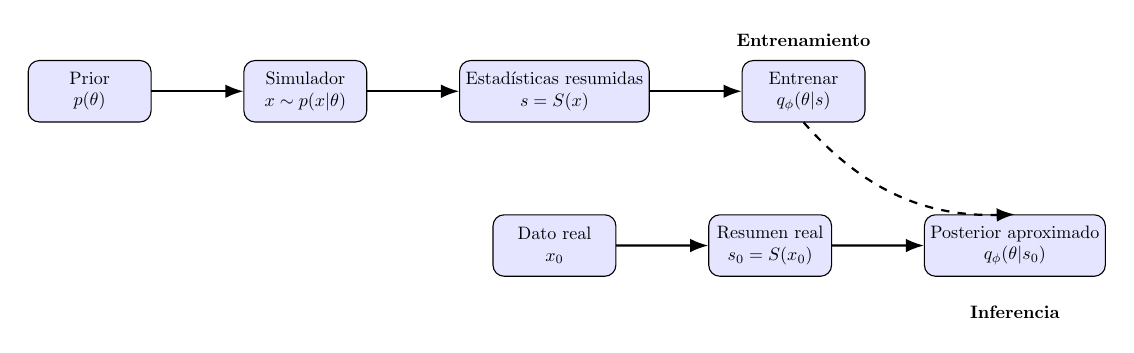
\begin{tikzpicture}[
        scale=0.65,  
        every node/.style={transform shape}, 
        node distance=1.2cm and 1.8cm,
        box/.style={draw, rounded corners, minimum width=2.4cm, minimum height=1.2cm, align=center, fill=blue!10},
        arrow/.style={-{Latex}, thick}
    ]
        \node[box] (prior) {Prior \\ \( p(\theta) \)};
        \node[box, right=of prior] (simulator) {Simulador \\ \( x \sim p(x|\theta) \)};
        \node[box, right=of simulator] (summary) {Estadísticas resumidas \\ \( s = S(x) \)};
        \node[box, right=of summary] (train) {Entrenar \\ \( q_\phi(\theta|s) \)};
        \node[box, below=1.8cm of summary] (obs) {Dato real \\ \( x_0 \)};
        \node[box, right=of obs] (s_obs) {Resumen real \\ \( s_0 = S(x_0) \)};
        \node[box, right=of s_obs] (posterior) {Posterior aproximado \\ \( q_\phi(\theta|s_0) \)};

        \draw[arrow] (prior) -- (simulator);
        \draw[arrow] (simulator) -- (summary);
        \draw[arrow] (summary) -- (train);
        \draw[arrow] (obs) -- (s_obs);
        \draw[arrow] (s_obs) -- (posterior);
        \draw[arrow, dashed] (train.south) to[bend right=25] (posterior.north);

        \node[above=0.15cm of train] {\textbf{Entrenamiento}};
        \node[below=0.45cm of posterior] {\textbf{Inferencia}};
    \end{tikzpicture}
    \caption{Pipeline general de SBI.}
    \label{fig:sbi}
\end{figure}

At vero eos et accusamus et iusto odio dignissimos ducimus qui blanditiis praesentium voluptatum deleniti atque corrupti quos dolores et quas molestias excepturi sint occaecati cupiditate non provident, similique sunt in culpa qui officia deserunt mollitia animi, id est laborum et dolorum fuga. Et harum quidem rerum facilis est et expedita distinctio. Nam libero tempore, cum soluta nobis est eligendi optio cumque nihil impedit quo minus id quod maxime placeat facere possimus, omnis voluptas assumenda est, omnis dolor repellendus. Temporibus autem quibusdam et aut officiis debitis aut rerum necessitatibus saepe eveniet ut et voluptates repudiandae sint et molestiae non recusandae. Itaque earum rerum hic tenetur a sapiente delectus, ut aut reiciendis voluptatibus maiores alias consequatur aut perferendis doloribus asperiores repellat



\end{document}